\begin{savequote}[8cm]
Far out in the uncharted backwaters of the unfashionable end of the western spiral arm of the Galaxy lies a small unregarded yellow sun. Orbiting this at a distance of roughly ninety-two million miles is an utterly insignificant little blue green planet whose ape-descended life forms are so amazingly primitive that they still think digital watches are a pretty neat idea.
  \qauthor{--- D. Adams, The Hitchhiker's Guide to the Galaxy}
\end{savequote}

\chapter{Introduction}\label{ch:1-intro}

\minitoc

This chapter explains the background and motivation for my project and introduces the two sub-projects I have been working on for the last year.


\section{Scope of the thesis}

\section{Background}
How do you design and assemble something on the nanoscale? Imagine building something with lego bricks; you choose the building blocks you want and use your hands to attach them where you want them to be. But for nanoscale objects it is difficult to have that level of control and more success has been had by instead imitating nature and letting the building blocks assemble themselves.

\subsection{DNA design}
Deoxyribonucleic acid (DNA) is a string-like molecule used to encode the genes of living systems \cite{calladine1997understanding}. These strings are made up of units called \emph{nucleotides}, consisting of the connecting sugar-phosphate backbone as well as one of four possible bases: \emph{adenine} (A), \emph{thymine} (T) \emph{cytosine} (C), and \emph{guanine} (G).

Through Watson-Crick base-pairing, ``A'' forms two hydrogen bonds with ``T'', while ``G'' forms three with ``C'', making DNA double-stranded. Each strand has a directionality, conventionally represented as going from the 3' to the 5' end of the strand, making the duplex anti-parallel.

The bases of the duplex are hydrophobic, while the sugars-phosphate backbone is hydrophilic, which means that the bases ``hides'' on the inside of the duplex to avoid contact with water molecules. However, backbone distance is about 6 Å (0.6 nm), while the bases would need to be at a distance of 3.3 Å (the thinkness of the base) to not leave any room for water \cite{calladine1997understanding}. To solve this, the DNA duplex forms a double helix structure with a radius of about 9 Å, placing everything at an energetically confortable distance.

While a single double helix is the most natural confirmation, it is possible for strands to branch into multiple junctions. For example, the Holliday junction is a junction between four double-helical arms, shown in Figure \ref{fig:holliday} in one of its possible configurations.

\begin{figure}
    \centering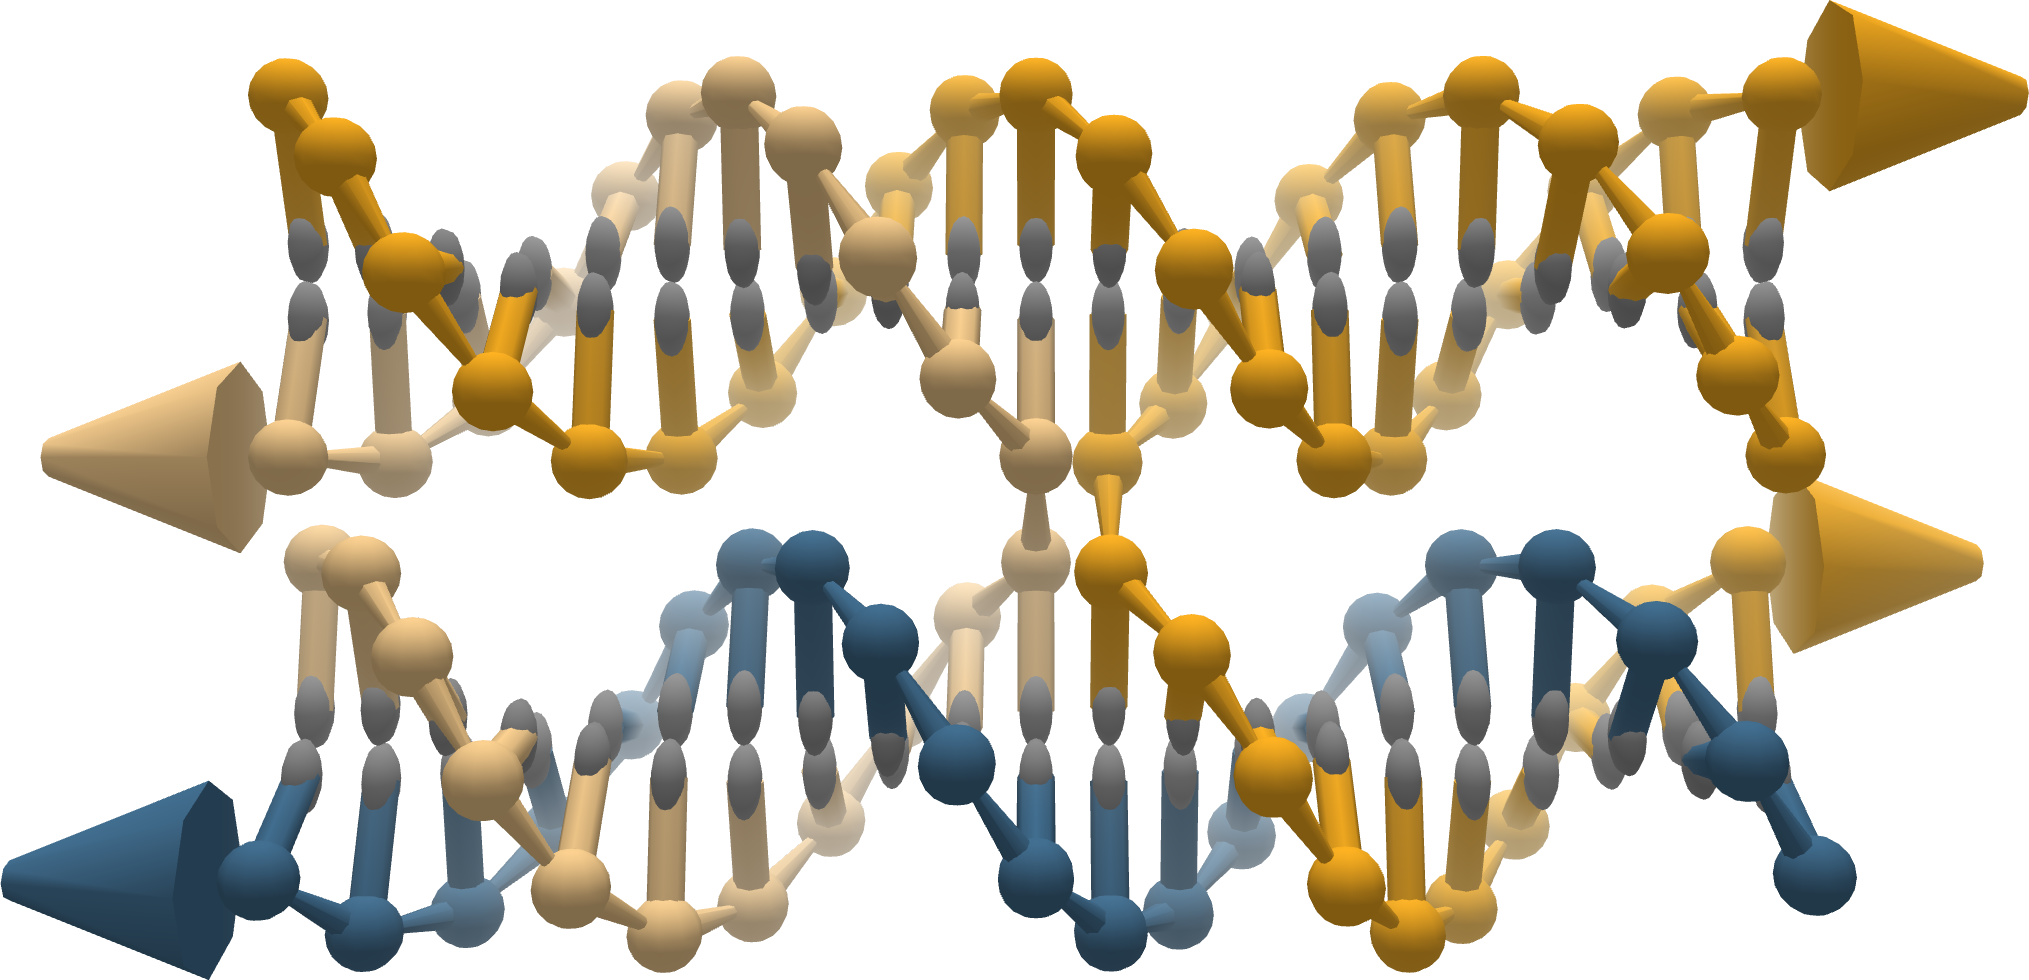
\includegraphics[width=\textwidth]{figures/holliday.png}
    \caption{Holliday junction, designed in oxView. Cones at the end indicates the 3' end of each of the four strands.}
    \label{fig:holliday}
\end{figure}

%https://www.rcsb.org/structure/1M6G

%Double-stranded DNA has a persistence lenght of approximately [], while single-stranded sections are much more flexible,

By designing sequences with complementary domains for the intended duplex regions, it is possible to create many different DNA motifs and structures \cite{seeman_2016}.

%% Add more here

A breakthrough in the field of structural DNA nanotechnology was the DNA origami tecnique \cite{rothemund2006folding} a now popular and proven method for creating larger irregular structures using DNA. The principle behind it, as illustrated in Figure \ref{fig:dnaOrigami}, is to use short staple strands to fold one long viral scaffold strand into the desired structure.

\begin{figure}
    \centering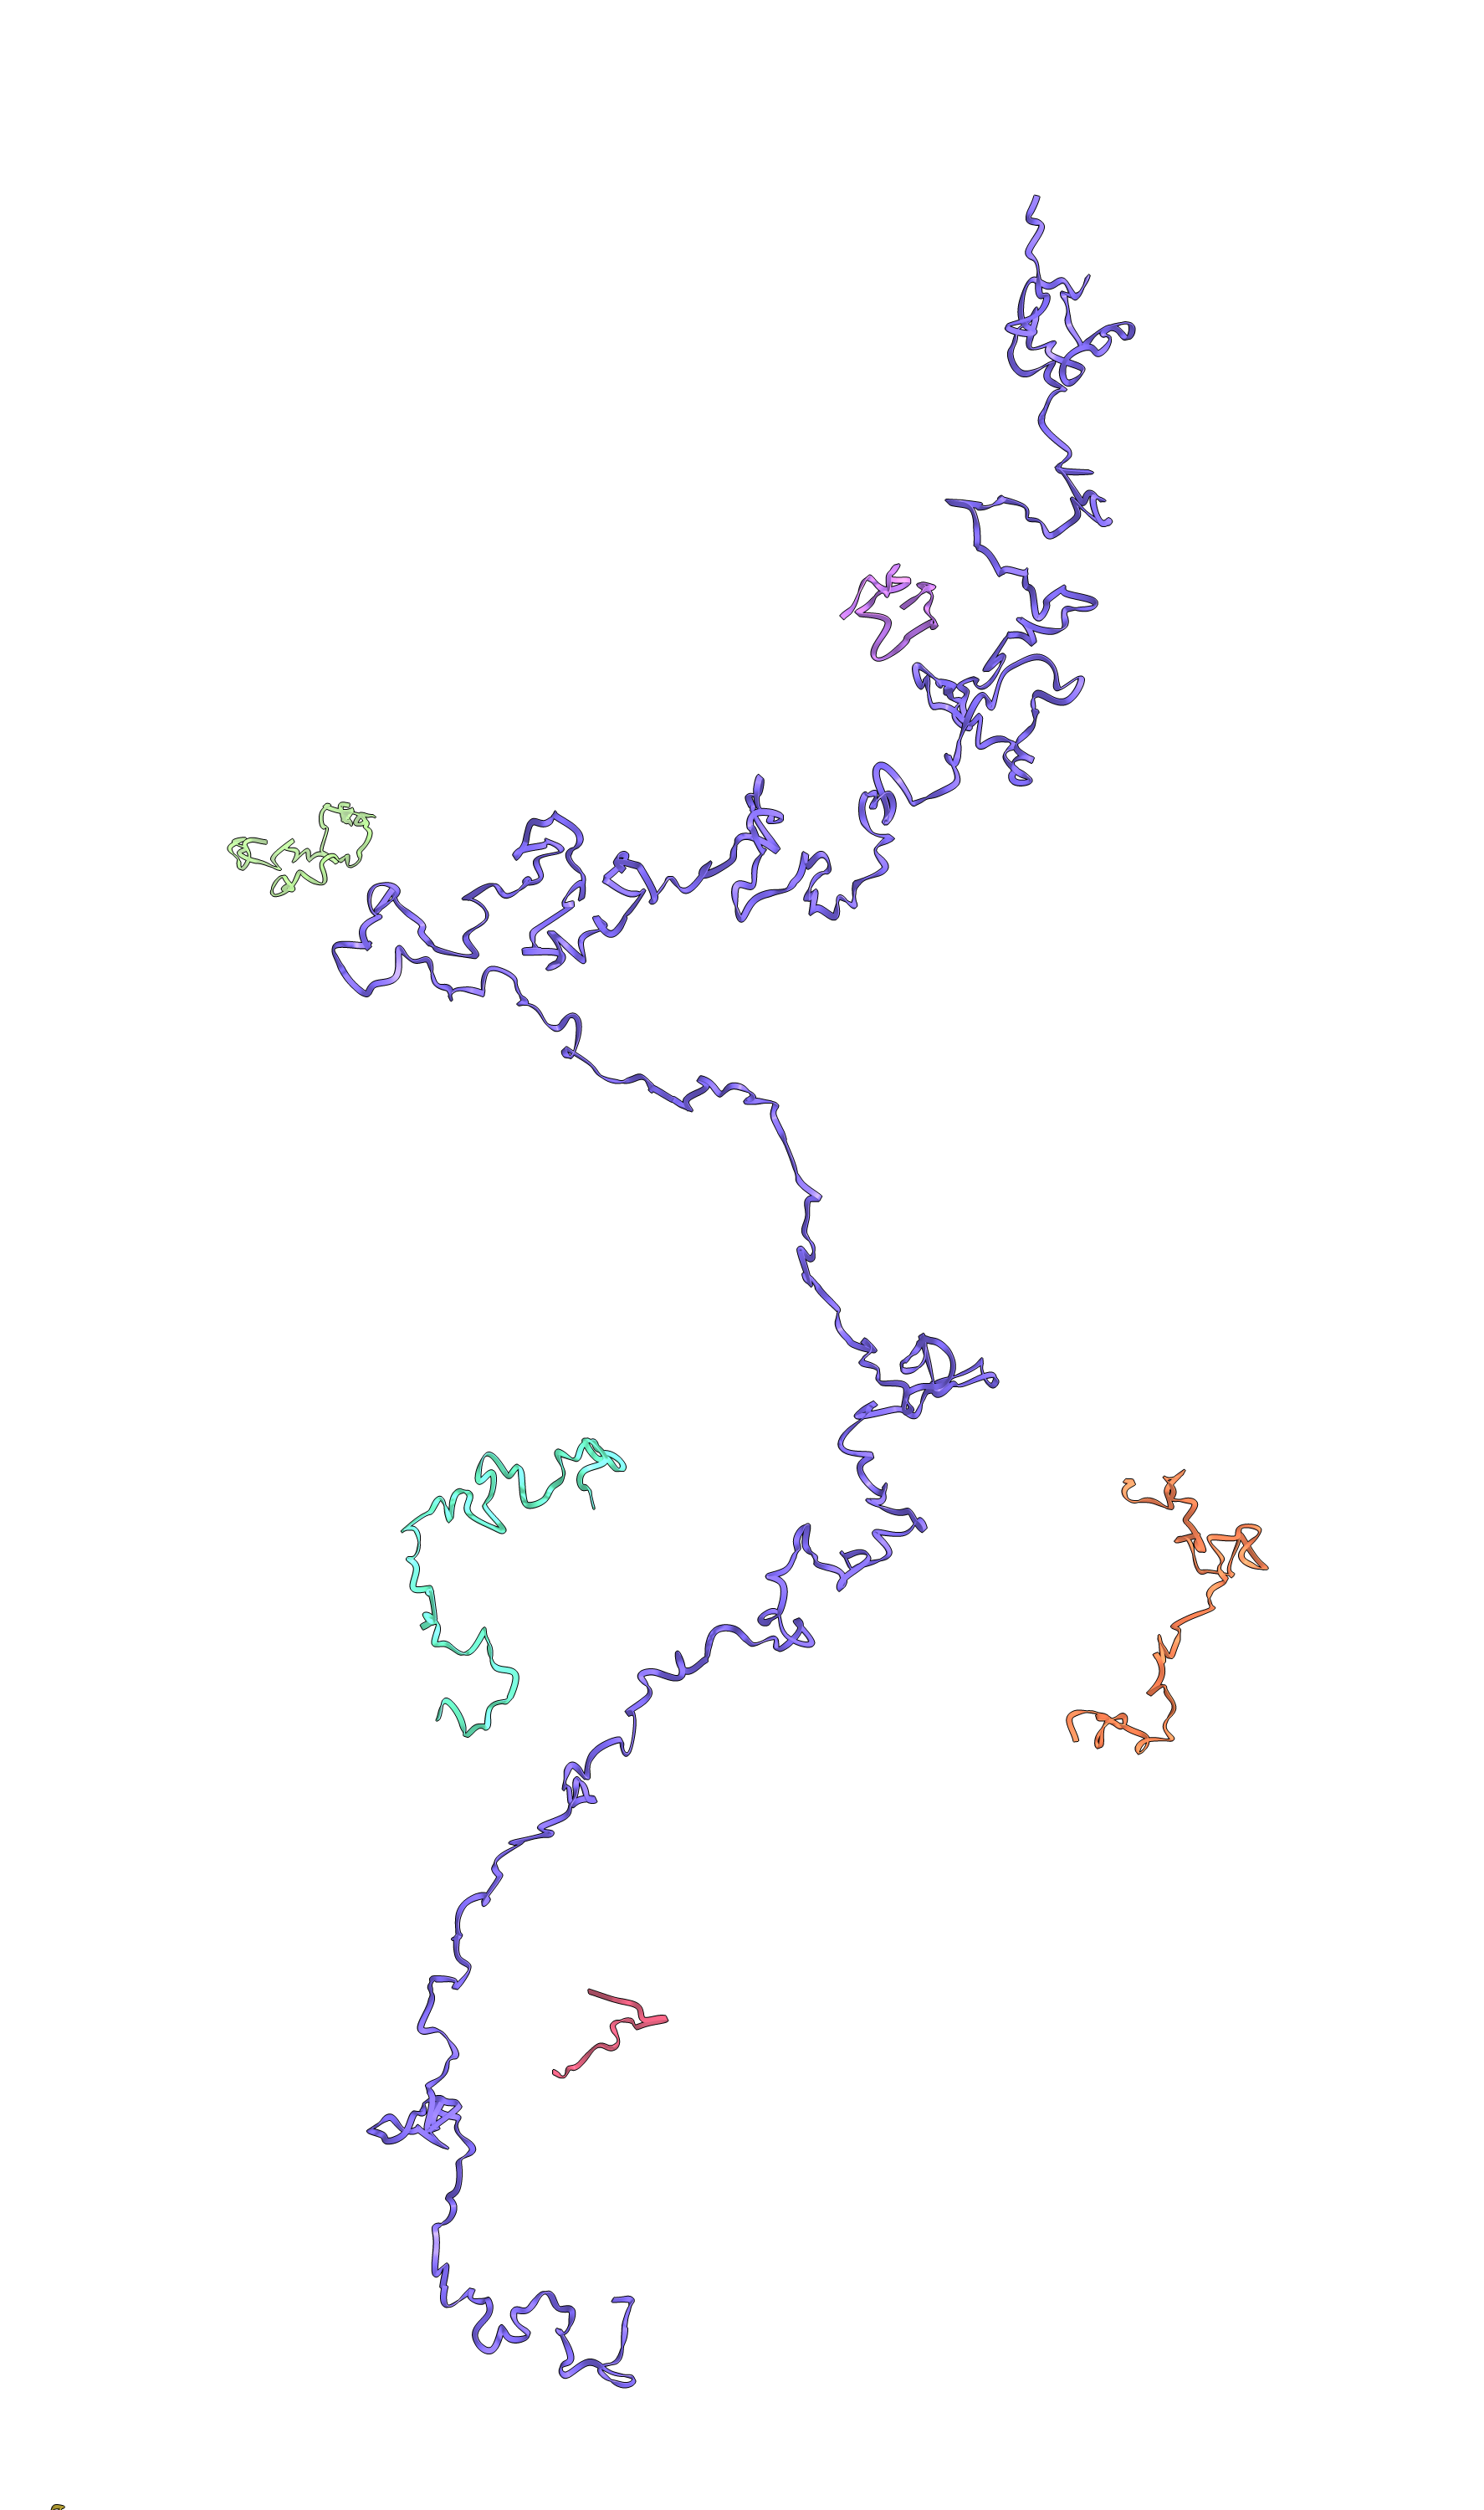
\includegraphics[width=\textwidth/5]{figures/melt/melted.png}\hfill
%    \centering\includegraphics[width=\textwidth/5]{figures/melt/intermediate2.png}\hfill
    \centering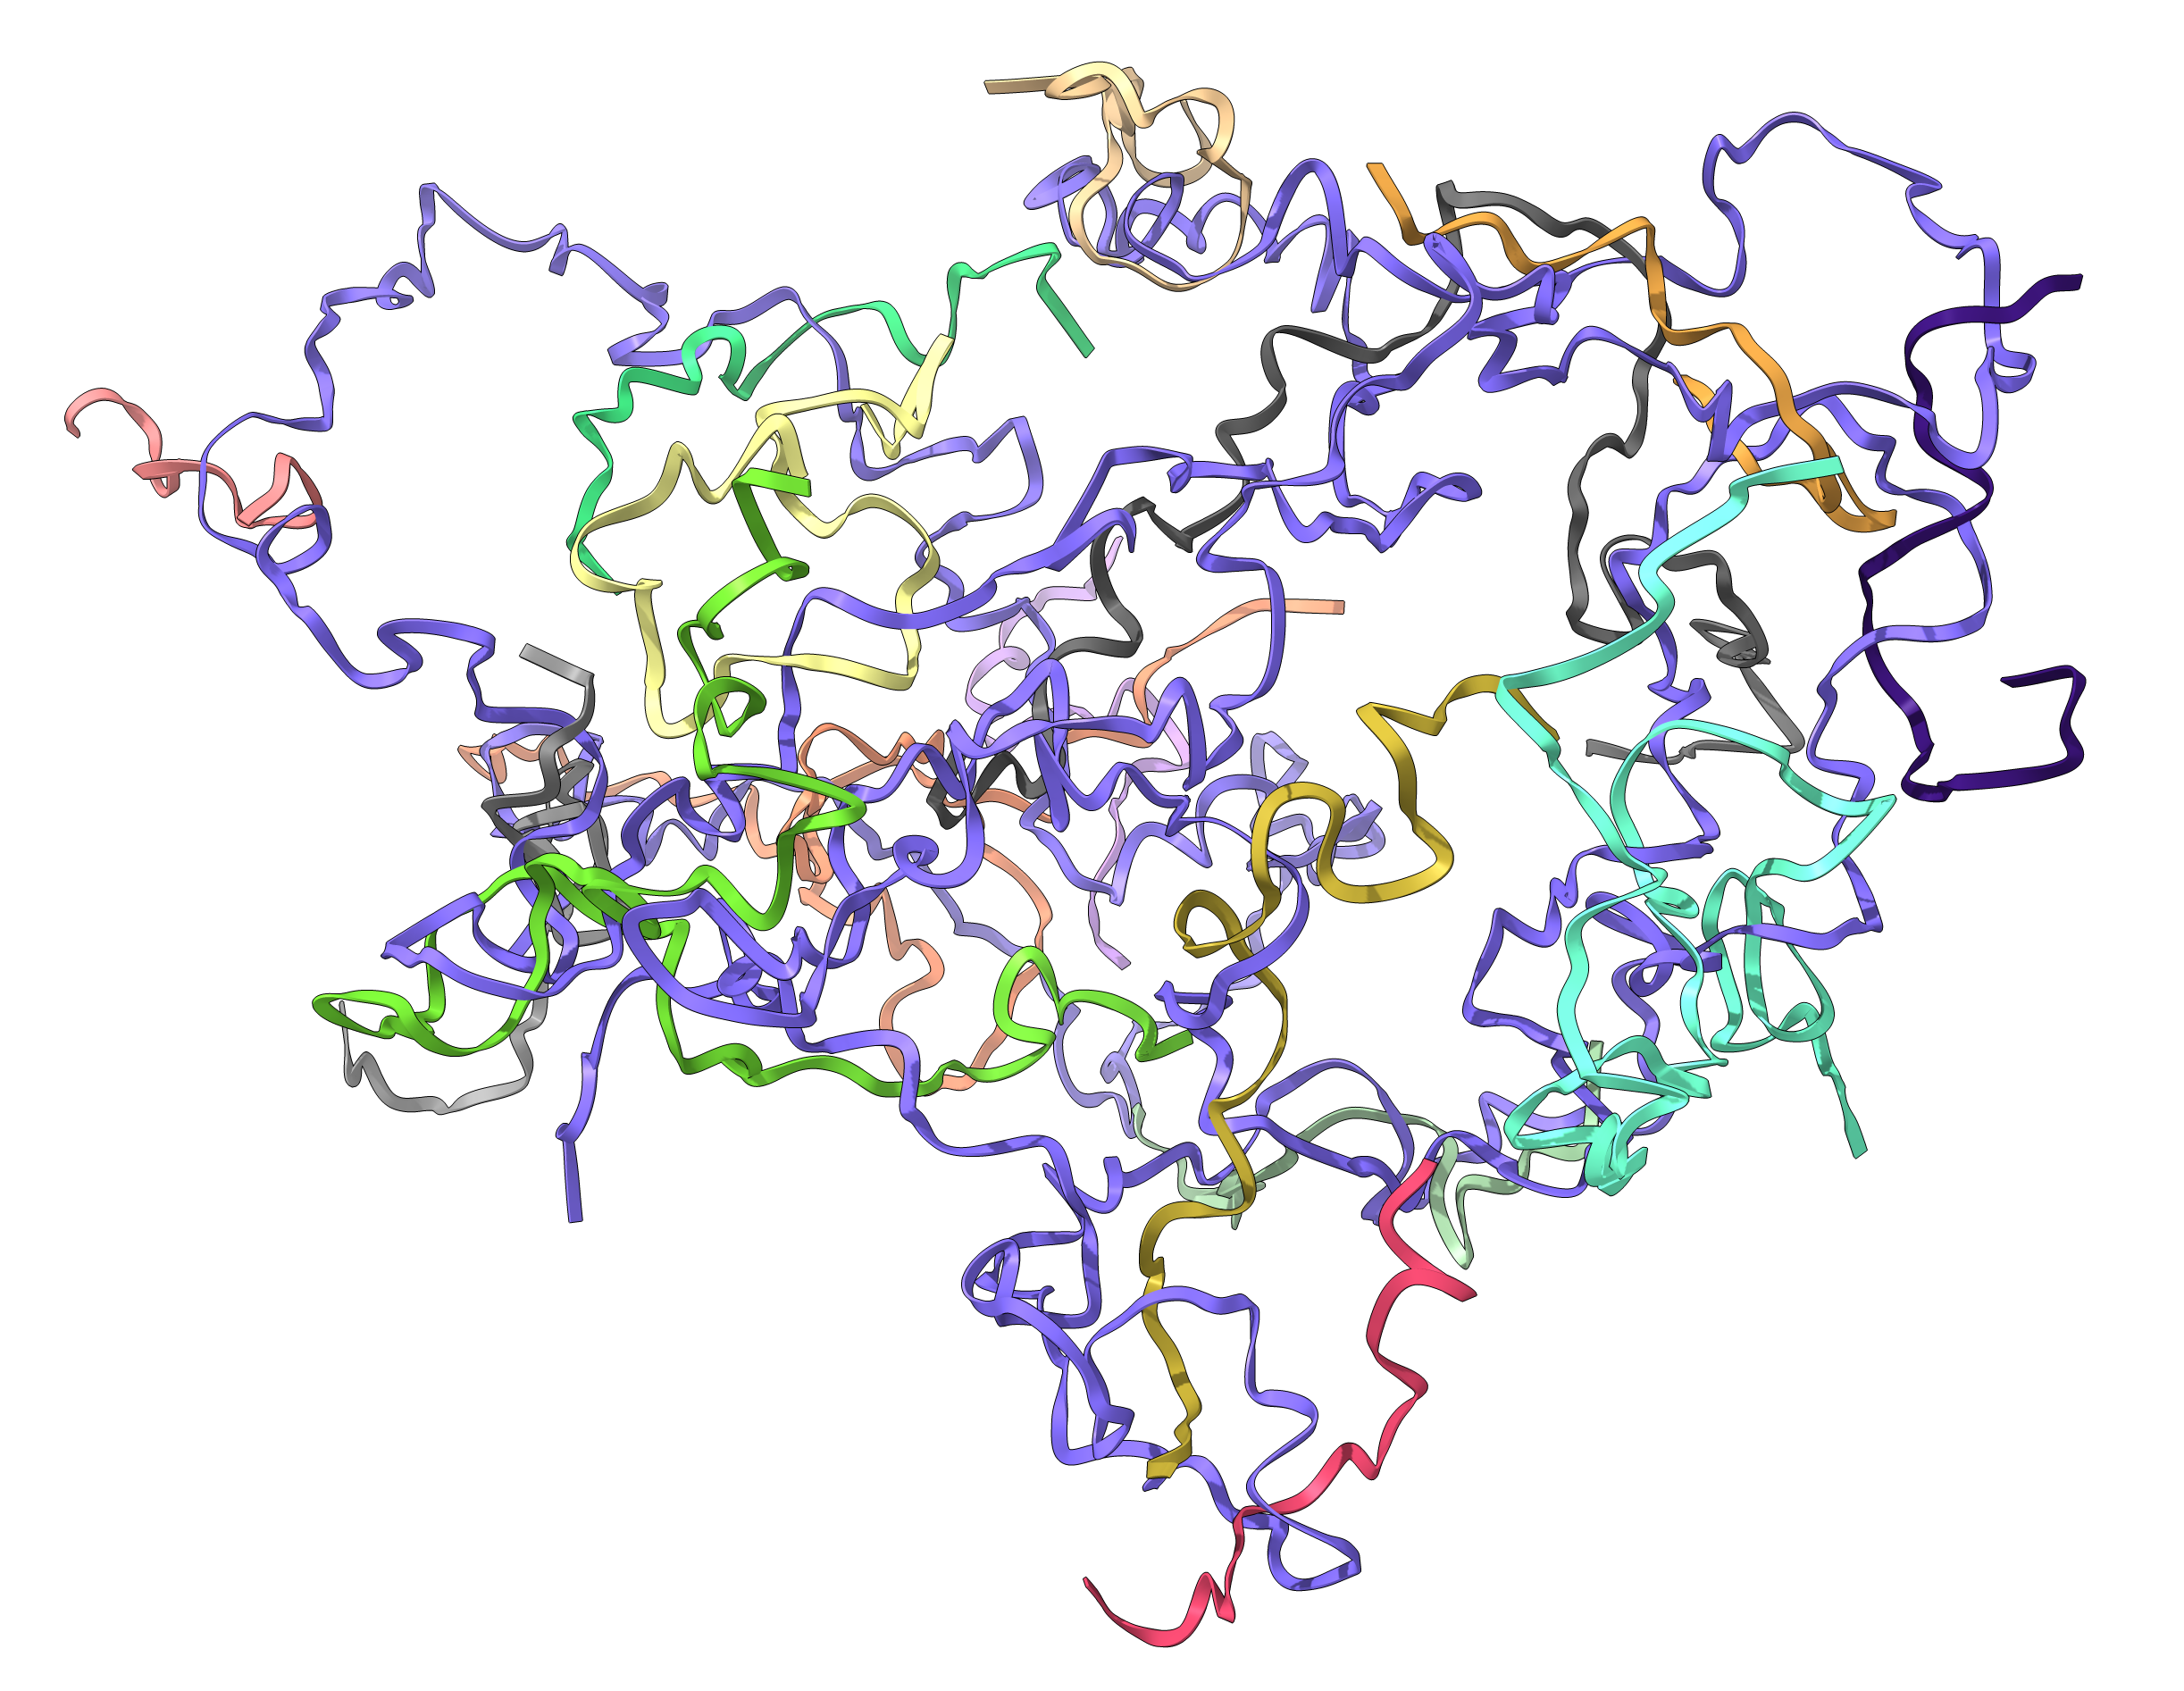
\includegraphics[width=\textwidth/3]{figures/melt/intermediate1.png}\hfill
    \centering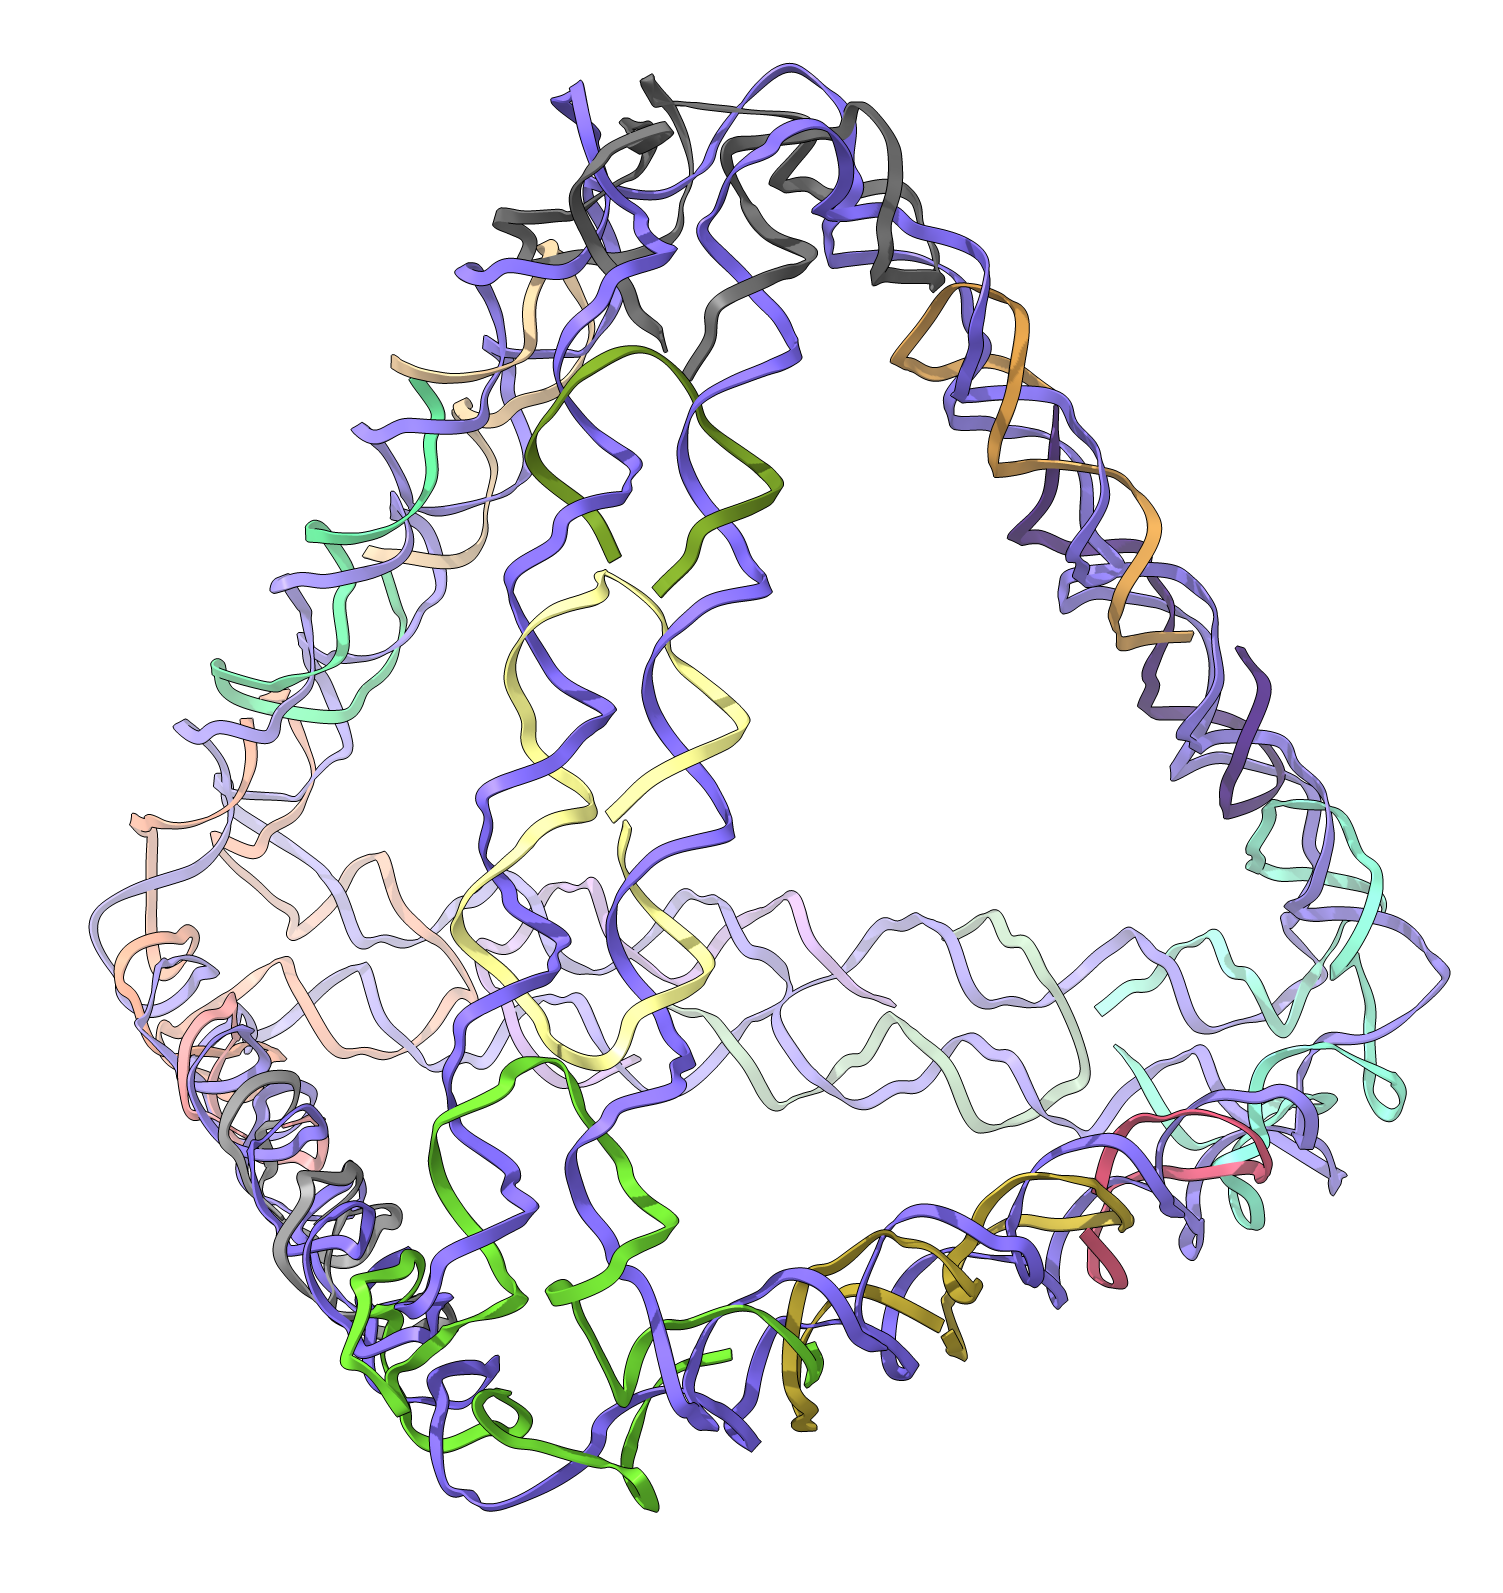
\includegraphics[width=\textwidth/3]{figures/melt/assembled.png}
    \caption{Illustration of DNA origami self-assembly of a tetrahedron. A long scaffold strand (purple), obtained from a virus, is folded into the desired shape by multiple short staple strands binding to complementary domains of the scaffold. Tetrahedron design obtained from \url{https://cando-dna-origami.org/examples/} and melted using oxDNA simulation \cite{ouldridge2010dna}.
    }
    \label{fig:dnaOrigami}
\end{figure}

Using design tools such as caDNAno\cite{douglas2009rapid}, it has become relatively easy to design structures of any given form. However, the size of the origami is limited by the length of the scaffold, which one of the motivations for researchers to investigate modular approaches, as described in Section \ref{sec:experimental_appl}.

\subsection{RNA design}
Ribonucleic acid (RNA) is very similar to DNA, but with the \emph{thymine} base replaced by \emph{uracil} (U). Biologically, DNA is transcribed into RNA by the RNA polymerase enzyme as part of gene expression, but just like DNA it is also possible to use RNA as a self-assembling building material.


Another possible building material investigated by the DNA robotics network is RNA. While DNA folding is easier to predict, the fact that RNA is more reactive also offers the possibility of a more useful structure; for example by incorporating aptamers, enzymes and other such functionalities\cite{guo2010emerging}.
Geary, et al., from the Andersen lab in Aarhus, demonstrated a method\cite{geary2014single, sparvath2017computer} for co-transcriptionally folded RNA origami in 2014, which also enables folding \emph{in vivo}. Using RNA origami, they were able to develop RNA tile modules, connecting through kissing-loop interactions. The Andersen lab is one of the network partners and I have spent a two-months secondment there working with their RNA origami method.

% "The emerging field of RNA nanotechnology121 might seem more promising in this regard because RNA is readily transcribed into a single strand in cells, which can be directly folded into a programmed nanostructure"
% https://www.nature.com/articles/nnano.2011.187

In order achieve my goal of improving the design of modular robotic structures, simulation tools are needed to analyse the assembly of both the complete structures and of each module. During the past year, I have been working with two related sub-projects to solve both those needs, each described in the following two sections.

